\documentclass[a4paper,12pt]{article}
\usepackage[latin1]{inputenc}
\usepackage[spanish]{babel}
\usepackage{bm}
\usepackage{graphicx}
\usepackage{amsmath}
\setlength{\textheight}{235mm}
\setlength{\textwidth}{168mm}
\setlength{\oddsidemargin}{0pt}
\pagestyle{empty}
\begin{document}
\mbox{}\vspace*{-45mm}

{\centering
{\small\sc Escuela T�cnica Superior de Ingenieros de Caminos, Canales y
Puertos (Madrid)}\\*[4mm]
{\Large\bf M�todo de los Elementos Finitos (Curso 23-24)}\\*[4mm]
Ejercicio 5: Modelos de viga y c�lculo est�tico\\*[4mm]

}

\vspace{3mm}

%%%%%
El p�rtico de dos vanos mostrado en la figura es de hormig�n armado con m�dulo de elasticidad $E=32$ GPa, coeficiente de Poisson $\nu=0.20$, y densidad de masa  $\rho=2548.42$ kg/m$^3$. Las secciones de las vigas son de $0.30$ m $\times$ $0.60$ m (base y altura), y las columnas tienen secci�n cuadrada de $0.40$ m de lado. Las cargas actuantes sobre la estructura son el peso propio del p�rtico, dos cargas puntuales verticales (en J y K), una carga puntual horizontal (en C) y una carga distribuida (sobre las vigas). Los apoyos A, D y G se consideran perfectamente empotrados. Los letras B, J, E, K y H indican la mitad de cada uno de los respectivos elementos estructurales.

Se pide realizar un modelo de vigas (considerar espacio 3D) con elementos tipo B31, tama�o de elementos $0.5$ m ($Global Seed/Approximate global size$) y responder las preguntas del cuestionario.

Las longitudes del p�rtico son tal como sigue: $l_{1}= 6$ m, $l_{2}= 5$ m, $l_{3}= 3$ m, $l_{4}$ y $l_{5}= 5$ m. Las cargas son $V_{1}= 70$ kN, $V_{2}= 50$ kN, $H_{1}= 488.40$ kN, y $q_{1}= 100$ kN/m. Las dimensiones de los elementos estructurales son $a= 0.40$ m, $b= 0.30$ m y $c= 0.60$ m.
\\
\begin{center}
	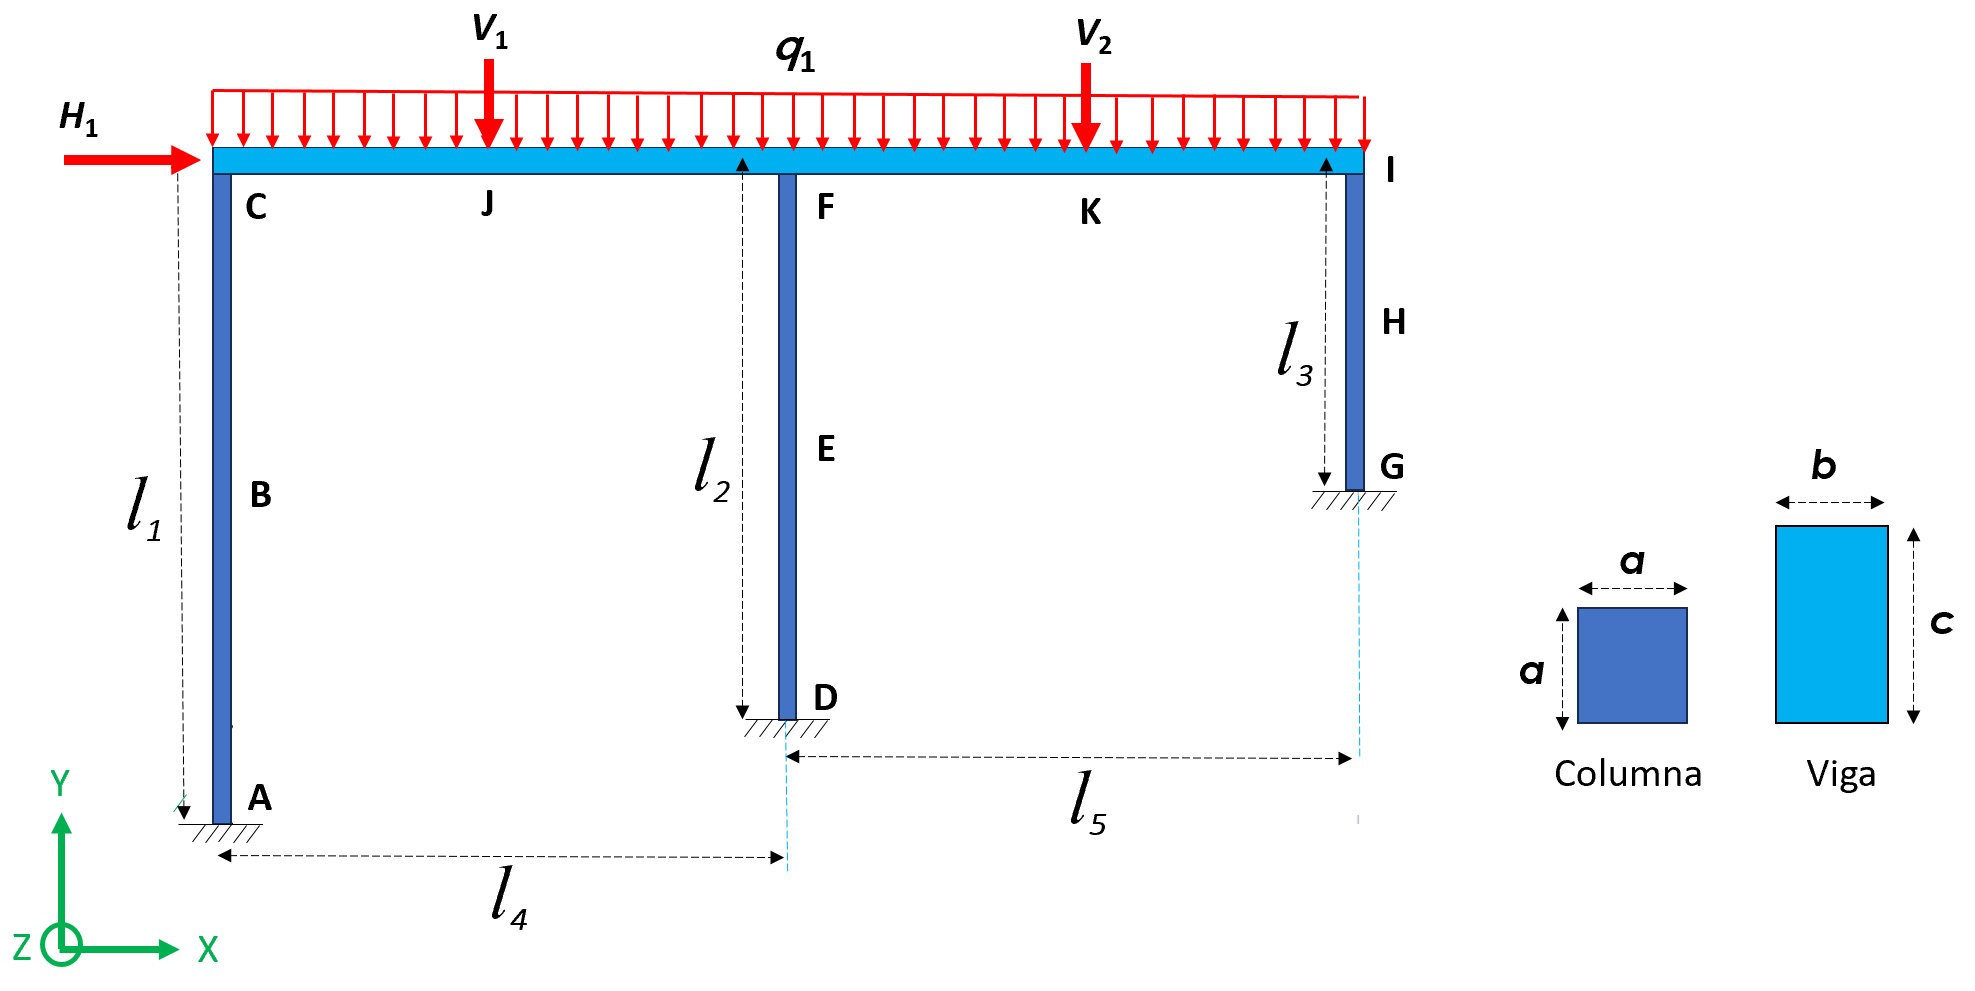
\includegraphics[width=1.05\textwidth]{figuraNT2023}
\end{center}
\end{document}
